% Section content template for individual Educative lessons
% This file contains the actual content for a specific section
% Generated from Educative API section content

% Section: Requirements of a Distributed Task Scheduler's Design
% Section ID: 6681764793942016
% Section Slug: requirements-of-a-distributed-task-schedulers-design
% Generated: 2025-12-07T22:09:04.464148

\subsection{Requirements}\label{m1N3FSFplPMTcV652JVYA}
\\
Let's start by understanding the functional and non-functional requirements for designing a task scheduler.

\subsubsection{Functional requirements}\label{iuloVafL_M0rGS46gEtbD}
\\
The functional requirements of the distributed task scheduler are as follows:

\begin{itemize}
\item
\protect\phantomsection\label{37WZqJRFzjCOWNUOIOND0}
\textbf{Submit tasks}: The system should allow the users to submit their tasks for execution.
\item
\protect\phantomsection\label{BQPjfXA0ZH0dfjoYkKWd7}
\textbf{Allocate resources}: The system should be able to allocate the required resources to each task.
\item
\protect\phantomsection\label{2mzUe7lqXfdoG_3ii9LGE}
\textbf{Remove tasks}: The system should allow the users to cancel the submitted tasks.
\item
\protect\phantomsection\label{sggGB0AEhebFqIqHLrcZb}
\textbf{Monitor task execution}: The task execution should be adequately monitored and rescheduled if the task fails to execute.
\item
\protect\phantomsection\label{JjuAGqUsJe11nqHgZtbmn}
\textbf{Efficient resource utilization}: The resources (CPU and memory) must be used efficiently in terms of time, cost, and fairness. Efficiency means that we do not waste resources. For example, if we allocate a heavy resource to a light task that can easily be executed on a cheap resource, it means that we have not efficiently utilized our resources. Fairness is all tenants' ability to get the resources with equally likely probability in a certain cost class.
\item
\protect\phantomsection\label{p7xKmA9B0Hw1z9RCZu2Bg}
\textbf{Release resources}: After successfully executing a task, the system should take back the resources assigned to the task.
\item
\protect\phantomsection\label{aTRx6ihbHU5pnOOZVnkzE}
\textbf{Show task status}: The system should show the users the current status of the task.
\end{itemize}

\begin{figure}[htbp]
 \centering
 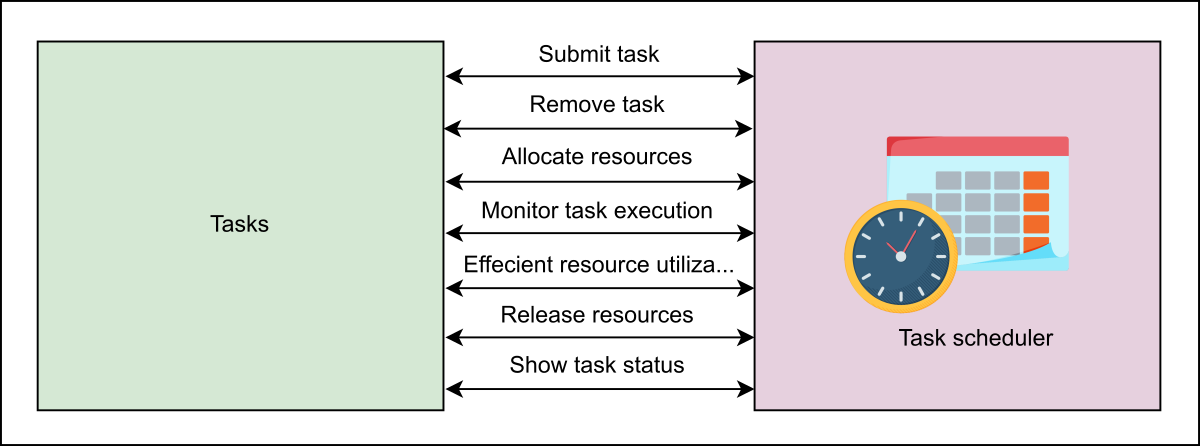
\includegraphics[width=0.5\textwidth]{Images/chapter_23/section_6681764793942016/5355432053178368.png}
 \caption{Functional requirements of the distributed task scheduler}
\end{figure}

\subsubsection{Non-functional requirements}\label{c9EDD2Kcbx6l4epnVBb3m}
\\
The non-functional requirements of the distributed task scheduler are as follows:

\begin{itemize}
\item
\protect\phantomsection\label{3_oZ8KTTU9UP3fNt0GHXn}
\textbf{Availability:} The system should be highly available to schedule and execute tasks.
\item
\protect\phantomsection\label{xOFi0xxDeKO-zpwftK5xP}
\textbf{Durability:} The tasks received by the system should be durable and should not be lost.
\item
\protect\phantomsection\label{8or45XCnM9enb1bjBaev5}
\textbf{Scalability:} The system should be able to schedule and execute an ever-increasing number of tasks per day.
\item
\protect\phantomsection\label{vqV8wFgRQbqnJOoo8KoGG}
\textbf{Fault-tolerance:} The system must be fault-tolerant by providing services uninterrupted despite faults in one or more of its components.
\item
\protect\phantomsection\label{pDSpkzwoSvYld5dCPrej5}
\textbf{Bounded waiting time:} This is how long a task needs to wait before starting execution. We must not execute tasks much later than expected. Users shouldn't be kept on waiting for an infinite time. If the waiting time for users crosses a certain threshold, they should be notified.
\end{itemize}

\begin{figure}[htbp]
 \centering
 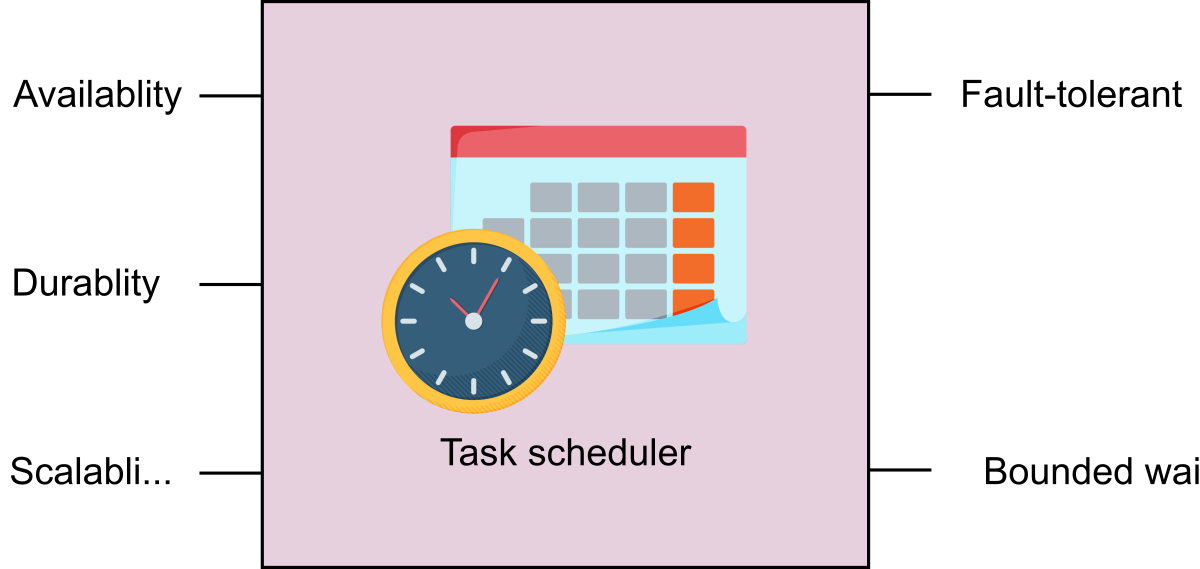
\includegraphics[width=0.5\textwidth]{Images/chapter_23/section_6681764793942016/6341000429961216.png}
 \caption{Non-functional requirements of distributed task scheduler}
\end{figure}

So far in this lesson, we have learned about task schedulers in general and distinguished between centralized and distributed task schedulers. Lastly , we listed the requirements of the distributed task scheduler system.

\subsection{Building blocks we will use}\label{Ki_3N3c0Z7gYcU_BUEWuN}
\\
We'll utilize the following building blocks in the design of our task scheduling system:

\begin{figure}[htbp]
 \centering
 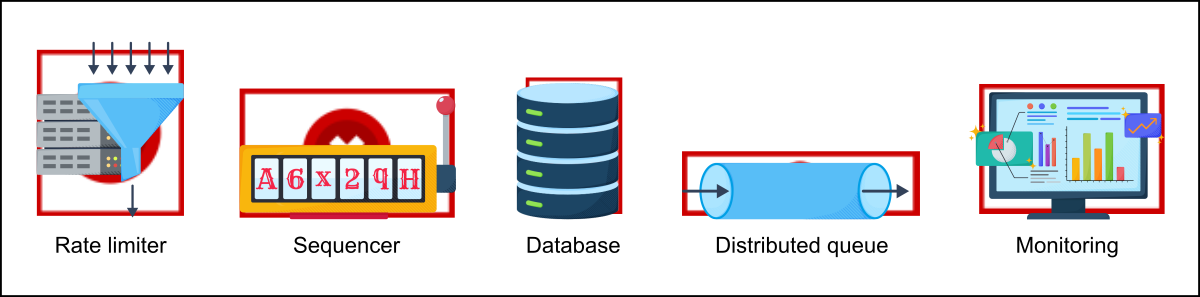
\includegraphics[width=0.5\textwidth]{Images/chapter_23/section_6681764793942016/5253970245582848.png}
 \caption{Building blocks of a task schedular}
\end{figure}

\begin{itemize}
\item
\protect\phantomsection\label{8raO21NJyJ_rARXXLet2q}
\href{https://www.educative.io/courses/grokking-the-system-design-interview/system-design-the-rate-limiter}{\textbf{Rate limiter}} is required to limit the number of tasks so that our system is reliable.
\item
\protect\phantomsection\label{8gJaOQwMzXQY9S3IoGsYF}
\href{https://www.educative.io/courses/grokking-the-system-design-interview/system-design-sequencer}{\textbf{A sequencer}} is needed to uniquely identify tasks.
\item
\protect\phantomsection\label{cGj5wO71SouFOrG674aQg}
\href{https://www.educative.io/courses/grokking-the-system-design-interview/introduction-to-databases}{\textbf{Database(s)}} are used to store task information.
\item
\protect\phantomsection\label{KpW0kXyhpiRTpkxQh6ds2}
\href{https://www.educative.io/courses/grokking-the-system-design-interview/system-design-the-distributed-messaging-queue}{\textbf{A distributed queue}} is required to arrange tasks in the order of execution.
\item
\protect\phantomsection\label{tRMxa24b0yG4QdhoWh7zY}
\href{https://www.educative.io/courses/grokking-the-system-design-interview/system-design-distributed-monitoring}{\textbf{Monitoring}} is essential to check the health of the resources and to detect failed tasks to provide reliable service to the users.
\end{itemize}
\\
We've identified the requirements of the task scheduler. In the next lesson, we'll design our task scheduling system according to these requirements.

% End of section content